\subsection{All panels}
\label{app:repro-panels}

\begin{table}[htbp]
    \centering
    \caption[Printed scale factors against the exact solution's]{\textbf{The exact solution reproduces the printed scale factor of every ordinary panel, to within one unit of the last printed digit, and of no partial differential or nonlinear panel.} Per panel of Wu et al.\ at their printed $n$: the printed scale factor $\eta$, the exact solution's $\eta_e=\|b\|^2$ ($b$, its Chebyshev coefficients; \Cref{eq:eta-e}) and the paper-faithful ground state's $\eta$. $^\dagger$Ground state not trusted (degenerate kernel, or gap ratio below 20). Classical computation.}
    \label{tab:eta-reproduction}
    \small
    \begin{tabular}{@{}l l r l l l l@{}}
        \toprule
        Fig. & Problem & $n$ & Printed $\eta$ & Ideal $\eta_e=\|b\|^2$ & Ground state & Agreement \\
        \midrule
        3b & R2a & 3 & 1.29 & \res[places=5]{build/R2a/faithful/standard/n3}{eta_ideal} & $\res[places=5]{build/R2a/faithful/standard/n3}{eta}\resflag{build/R2a/faithful/standard/n3}{trusted}{}{^{\dagger}}$ & \checkmark \\
        3c & R2b & 3 & 32.47 & \res[places=5]{build/R2b/faithful/standard/n3}{eta_ideal} & $\res[places=5]{build/R2b/faithful/standard/n3}{eta}\resflag{build/R2b/faithful/standard/n3}{trusted}{}{^{\dagger}}$ & \checkmark (one unit low) \\
        3d & R2c & 5 & 451.71 & \res[places=5]{build/R2c/faithful/standard/n5}{eta_ideal} & $\res[places=5]{build/R2c/faithful/standard/n5}{eta}\resflag{build/R2c/faithful/standard/n5}{trusted}{}{^{\dagger}}$ & \checkmark \\
        4a & R3a & 3 & 1.75 & \res[places=5]{build/R3a/faithful/standard/n3}{eta_ideal} & $\res[places=5]{build/R3a/faithful/standard/n3}{eta}\resflag{build/R3a/faithful/standard/n3}{trusted}{}{^{\dagger}}$ & \checkmark \\
        4b & R3b & 3 & 1.49 & \res[places=5]{build/R3b/faithful/standard/n3}{eta_ideal} & $\res[places=5]{build/R3b/faithful/standard/n3}{eta}\resflag{build/R3b/faithful/standard/n3}{trusted}{}{^{\dagger}}$ & \checkmark \\
        4c & R3c & 5 & 108.51 & \res[places=5]{build/R3c/faithful/standard/n5}{eta_ideal} & $\res[places=5]{build/R3c/faithful/standard/n5}{eta}\resflag{build/R3c/faithful/standard/n5}{trusted}{}{^{\dagger}}$ & \checkmark \\
        4d & R3d & 5 & 135.38 & \res[places=5]{build/R3d/faithful/standard/n5}{eta_ideal} & $\res[places=5]{build/R3d/faithful/standard/n5}{eta}\resflag{build/R3d/faithful/standard/n5}{trusted}{}{^{\dagger}}$ & \checkmark \\
        5a & R4a & 3 & 1.35 & \res[places=5]{build/R4a/faithful/standard/n3}{eta_ideal} & $\res[places=5]{build/R4a/faithful/standard/n3}{eta}\resflag{build/R4a/faithful/standard/n3}{trusted}{}{^{\dagger}}$ & \checkmark \\
        5b & R4b & 3 & 14.74 & \res[places=5]{build/R4b/faithful/standard/n3}{eta_ideal} & $\res[places=5]{build/R4b/faithful/standard/n3}{eta}\resflag{build/R4b/faithful/standard/n3}{trusted}{}{^{\dagger}}$ & \checkmark (one unit low) \\
        5c & R4c & 4 & 0.82 & \res[places=5]{build/R4c/faithful/standard/n4}{eta_ideal} & $\res[places=5]{build/R4c/faithful/standard/n4}{eta}\resflag{build/R4c/faithful/standard/n4}{trusted}{}{^{\dagger}}$ & \checkmark \\
        5d & R4d & 4 & 77.51 & \res[places=5]{build/R4d/faithful/standard/n4}{eta_ideal} & $\res[places=5]{build/R4d/faithful/standard/n4}{eta}\resflag{build/R4d/faithful/standard/n4}{trusted}{}{^{\dagger}}$ & \checkmark \\
        \midrule
        6b & R5a & 3 & 5.21559 & \res[places=5]{build/R5a/faithful/standard/n3x3}{eta_ideal} & $\res[places=5]{build/R5a/faithful/standard/n3x3}{eta}\resflag{build/R5a/faithful/standard/n3x3}{trusted}{}{^{\dagger}}$ & $\times$ \\
        6d & R5b & 4 & 603.863 & \res[places=5]{build/R5b/faithful/standard/n4x4}{eta_ideal} & $\res[places=5]{build/R5b/faithful/standard/n4x4}{eta}\resflag{build/R5b/faithful/standard/n4x4}{trusted}{}{^{\dagger}}$ & $\times$ \\
        6f & R5c & 5 & 216.469 & \res[places=5]{build/R5c/faithful/standard/n5x5}{eta_ideal} & $\res[places=5]{build/R5c/faithful/standard/n5x5}{eta}\resflag{build/R5c/faithful/standard/n5x5}{trusted}{}{^{\dagger}}$ & $\times$ \\
        7b & R6a & 2 & 3.75367 & \res[places=5]{build/R6a/faithful/standard/n2}{eta_ideal} & $\res[places=5]{build/R6a/faithful/standard/n2}{eta}\resflag{build/R6a/faithful/standard/n2}{trusted}{}{^{\dagger}}$ & $\times$ \\
        7c & R6b & 2 & 0.07984 & \res[places=5]{build/R6b/faithful/standard/n2}{eta_ideal} & $\res[places=5]{build/R6b/faithful/standard/n2}{eta}\resflag{build/R6b/faithful/standard/n2}{trusted}{}{^{\dagger}}$ & $\times$ \\
        \bottomrule
    \end{tabular}
\end{table}

\begin{table}[htbp]
    \centering
    \caption[Errors of Wu et al.'s solutions, as printed and as run]{\textbf{Errors of Wu et al.'s solutions at the printed resolution, as printed and as run.} $L^\infty$ error of each panel as printed (the paper-faithful variant) and of the problem as run, at the printed $n$, and the problem's least error over $n$; on 1001 points ($101\times101$ on two axes). $^\dagger$Ground state not trusted (degenerate kernel, or gap ratio below 20); --, the doubled space (R6), whose kernel is never trusted. Classical computation.}
    \label{tab:app-repro-errors}
    \small
    \begin{tabular}{@{}l l r l l l@{}}
        \toprule
        Fig. & Problem & Printed $n$ & As printed & As run & As run, best over $n$ \\
        \midrule
        3b & R2a & 3 & $\res[2,sci]{build/R2a/faithful/standard/n3}{field_err_linf}\resflag{build/R2a/faithful/standard/n3}{trusted}{}{^{\dagger}}$ & $\res[2,sci]{build/R2a/standard/n3}{field_err_linf}\resflag{build/R2a/standard/n3}{trusted}{}{^{\dagger}}$ & \res[2,sci]{build/R2a/standard/best}{field_err_linf} ($n = \res{build/R2a/standard/best}{n}$) \\
        3c & R2b & 3 & $\res[2,sci]{build/R2b/faithful/standard/n3}{field_err_linf}\resflag{build/R2b/faithful/standard/n3}{trusted}{}{^{\dagger}}$ & $\res[2,sci]{build/R2b/standard/n3}{field_err_linf}\resflag{build/R2b/standard/n3}{trusted}{}{^{\dagger}}$ & \res[2,sci]{build/R2b/standard/best}{field_err_linf} ($n = \res{build/R2b/standard/best}{n}$) \\
        3d & R2c & 5 & $\res[2,sci]{build/R2c/faithful/standard/n5}{field_err_linf}\resflag{build/R2c/faithful/standard/n5}{trusted}{}{^{\dagger}}$ & $\res[2,sci]{build/R2c/standard/n5}{field_err_linf}\resflag{build/R2c/standard/n5}{trusted}{}{^{\dagger}}$ & \res[2,sci]{build/R2c/standard/best}{field_err_linf} ($n = \res{build/R2c/standard/best}{n}$) \\
        4a & R3a & 3 & $\res[2,sci]{build/R3a/faithful/standard/n3}{field_err_linf}\resflag{build/R3a/faithful/standard/n3}{trusted}{}{^{\dagger}}$ & $\res[2,sci]{build/R3a/standard/n3}{field_err_linf}\resflag{build/R3a/standard/n3}{trusted}{}{^{\dagger}}$ & \res[2,sci]{build/R3a/standard/best}{field_err_linf} ($n = \res{build/R3a/standard/best}{n}$) \\
        4b & R3b & 3 & $\res[2,sci]{build/R3b/faithful/standard/n3}{field_err_linf}\resflag{build/R3b/faithful/standard/n3}{trusted}{}{^{\dagger}}$ & $\res[2,sci]{build/R3b/standard/n3}{field_err_linf}\resflag{build/R3b/standard/n3}{trusted}{}{^{\dagger}}$ & \res[2,sci]{build/R3b/standard/best}{field_err_linf} ($n = \res{build/R3b/standard/best}{n}$) \\
        4c & R3c & 5 & $\res[2,sci]{build/R3c/faithful/standard/n5}{field_err_linf}\resflag{build/R3c/faithful/standard/n5}{trusted}{}{^{\dagger}}$ & $\res[2,sci]{build/R3c/standard/n5}{field_err_linf}\resflag{build/R3c/standard/n5}{trusted}{}{^{\dagger}}$ & \res[2,sci]{build/R3c/standard/best}{field_err_linf} ($n = \res{build/R3c/standard/best}{n}$) \\
        4d & R3d & 5 & $\res[2,sci]{build/R3d/faithful/standard/n5}{field_err_linf}\resflag{build/R3d/faithful/standard/n5}{trusted}{}{^{\dagger}}$ & $\res[2,sci]{build/R3d/standard/n5}{field_err_linf}\resflag{build/R3d/standard/n5}{trusted}{}{^{\dagger}}$ & \res[2,sci]{build/R3d/standard/best}{field_err_linf} ($n = \res{build/R3d/standard/best}{n}$) \\
        5a & R4a & 3 & $\res[2,sci]{build/R4a/faithful/standard/n3}{field_err_linf}\resflag{build/R4a/faithful/standard/n3}{trusted}{}{^{\dagger}}$ & $\res[2,sci]{build/R4a/standard/n3}{field_err_linf}\resflag{build/R4a/standard/n3}{trusted}{}{^{\dagger}}$ & \res[2,sci]{build/R4a/standard/best}{field_err_linf} ($n = \res{build/R4a/standard/best}{n}$) \\
        5b & R4b & 3 & $\res[2,sci]{build/R4b/faithful/standard/n3}{field_err_linf}\resflag{build/R4b/faithful/standard/n3}{trusted}{}{^{\dagger}}$ & $\res[2,sci]{build/R4b/standard/n3}{field_err_linf}\resflag{build/R4b/standard/n3}{trusted}{}{^{\dagger}}$ & \res[2,sci]{build/R4b/standard/best}{field_err_linf} ($n = \res{build/R4b/standard/best}{n}$) \\
        5c & R4c & 4 & $\res[2,sci]{build/R4c/faithful/standard/n4}{field_err_linf}\resflag{build/R4c/faithful/standard/n4}{trusted}{}{^{\dagger}}$ & $\res[2,sci]{build/R4c/standard/n4}{field_err_linf}\resflag{build/R4c/standard/n4}{trusted}{}{^{\dagger}}$ & \res[2,sci]{build/R4c/standard/best}{field_err_linf} ($n = \res{build/R4c/standard/best}{n}$) \\
        5d & R4d & 4 & $\res[2,sci]{build/R4d/faithful/standard/n4}{field_err_linf}\resflag{build/R4d/faithful/standard/n4}{trusted}{}{^{\dagger}}$ & $\res[2,sci]{build/R4d/standard/n4}{field_err_linf}\resflag{build/R4d/standard/n4}{trusted}{}{^{\dagger}}$ & \res[2,sci]{build/R4d/standard/best}{field_err_linf} ($n = \res{build/R4d/standard/best}{n}$) \\
        6b & R5a & 3 & $\res[2,sci]{build/R5a/faithful/standard/n3x3}{field_err_linf}\resflag{build/R5a/faithful/standard/n3x3}{trusted}{}{^{\dagger}}$ & $\res[2,sci]{build/R5a/standard/n3x3}{field_err_linf}\resflag{build/R5a/standard/n3x3}{trusted}{}{^{\dagger}}$ & \res[2,sci]{build/R5a/standard/best}{field_err_linf} ($n = \res{build/R5a/standard/best}{n}$) \\
        6d & R5b & 4 & $\res[2,sci]{build/R5b/faithful/standard/n4x4}{field_err_linf}\resflag{build/R5b/faithful/standard/n4x4}{trusted}{}{^{\dagger}}$ & $\res[2,sci]{build/R5b/standard/n4x4}{field_err_linf}\resflag{build/R5b/standard/n4x4}{trusted}{}{^{\dagger}}$ & \res[2,sci]{build/R5b/standard/best}{field_err_linf} ($n = \res{build/R5b/standard/best}{n}$) \\
        6f & R5c & 5 & $\res[2,sci]{build/R5c/faithful/standard/n5x5}{field_err_linf}\resflag{build/R5c/faithful/standard/n5x5}{trusted}{}{^{\dagger}}$ & $\res[2,sci]{build/R5c/standard/n5x5}{field_err_linf}\resflag{build/R5c/standard/n5x5}{trusted}{}{^{\dagger}}$ & \res[2,sci]{build/R5c/standard/best}{field_err_linf} ($n = \res{build/R5c/standard/best}{n}$) \\
        7b & R6a & 2 & $\res[2,sci]{build/R6a/faithful/standard/n2}{field_err_linf}\resflag{build/R6a/faithful/standard/n2}{trusted}{}{^{\dagger}}$ & $\res[2,sci]{build/R6a/standard/n2}{field_err_linf}\resflag{build/R6a/standard/n2}{trusted}{}{^{\dagger}}$ & -- \\
        7c & R6b & 2 & $\res[2,sci]{build/R6b/faithful/standard/n2}{field_err_linf}\resflag{build/R6b/faithful/standard/n2}{trusted}{}{^{\dagger}}$ & $\res[2,sci]{build/R6b/standard/n2}{field_err_linf}\resflag{build/R6b/standard/n2}{trusted}{}{^{\dagger}}$ & -- \\
        \bottomrule
    \end{tabular}
\end{table}

\subsection{The Fig.~5 triage}
\label{app:repro-triage}

\begin{figure}[htbp]
    \centering
    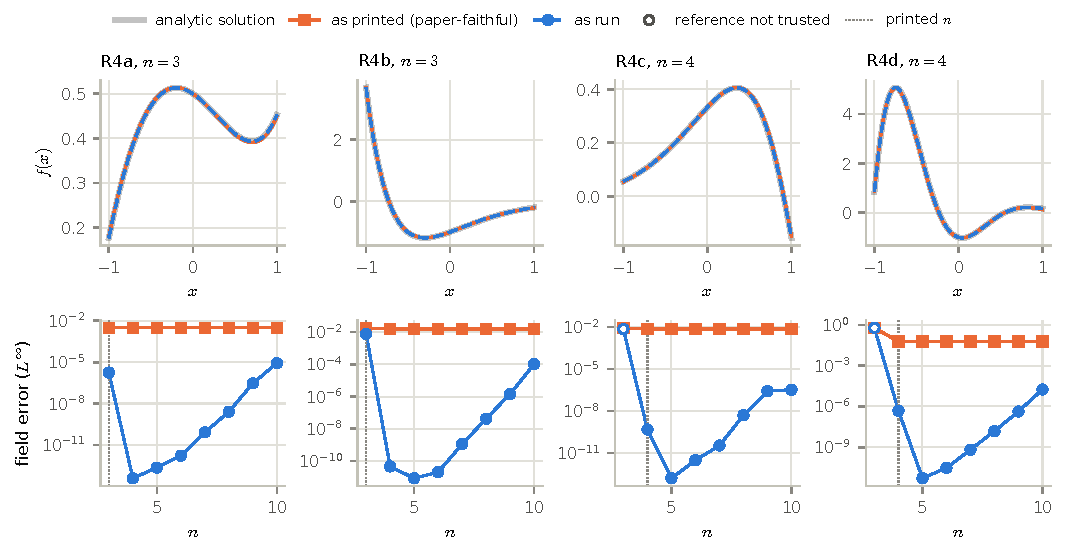
\includegraphics[width=\linewidth]{Figs/faithful_vs_corrected.pdf}
    \caption[The paper-faithful variant against the problems as run, Fig.~5]{\textbf{As printed, each panel of Wu et al.'s Fig.~5 holds at an error floor that no resolution removes; as run, it converges spectrally.} R4a--R4d. Top: the analytic solution, the paper-faithful ground state (rounded constraint point, Maclaurin source) and the problem as run (exact root, Chebyshev source) at the printed $n$; the three coincide at plot scale, the paper-faithful errors there lying between $\res[2,sci]{build/R4a/faithful/standard/n3}{field_err_linf}$ (R4a) and $\res[2,sci]{build/R4d/faithful/standard/n4}{field_err_linf}$ (R4d). Bottom: the $L^\infty$ field error against $n$ for both variants (open where the reference is not trusted), the printed $n$ dotted. The paper-faithful error holds at its floor (\Cref{tab:app-fig5-triage}); as run it falls to between $\res[2,sci]{build/R4a/standard/best}{field_err_linf}$ and $\res[2,sci]{build/R4b/standard/best}{field_err_linf}$ at $n=4$ or $5$, then rises with the standard form's conditioning (\Cref{prop:wedin}). On R4b the printed $n=3$ is itself under-resolved: as run, the error there is $\res[2,sci]{build/R4b/standard/n3}{field_err_linf}$. Classical computation (dense \gls{svd}).}
    \label{fig:faithful-vs-corrected}
\end{figure}

\begin{table}[htbp]
    \centering
    \caption[The printed choices behind the error of Wu et al.'s Fig.~5]{\textbf{Each printed choice alone sets an error floor; only both departures together converge.} $L^\infty$ error on Wu et al.'s Fig.~5 panels over $n=4,\dots,10$: the paper-faithful variant (rounded constraint point, Maclaurin source), each departure alone (exact root; Chebyshev source coefficients), and both together at their best $n$. --, R4a's polynomial source is already exact, so its rounded point acts alone. Classical computation.}
    \label{tab:app-fig5-triage}
    \small
    \begin{tabular}{@{}l l l l l l@{}}
        \toprule
        Fig. & Problem & Faithful & Exact root & Chebyshev source & Both, best \\
        \midrule
        5a & R4a & \res[2,sci]{build/R4a/faithful/standard/floor}{low} & -- & -- & \res[2,sci]{build/R4a/standard/best}{field_err_linf} ($n = \res{build/R4a/standard/best}{n}$) \\
        5b & R4b & \res[2,sci]{build/R4b/faithful/standard/floor}{low} & \res[2,sci]{build/R4b/faithful/standard/floor/exact-root}{low} & \res[2,sci]{build/R4b/faithful/standard/floor/chebyshev-source}{low} & \res[2,sci]{build/R4b/standard/best}{field_err_linf} ($n = \res{build/R4b/standard/best}{n}$) \\
        5c & R4c & \res[2,sci]{build/R4c/faithful/standard/floor}{low} & \res[2,sci]{build/R4c/faithful/standard/floor/exact-root}{low} & \res[2,sci]{build/R4c/faithful/standard/floor/chebyshev-source}{low} & \res[2,sci]{build/R4c/standard/best}{field_err_linf} ($n = \res{build/R4c/standard/best}{n}$) \\
        5d & R4d & \res[2,sci]{build/R4d/faithful/standard/floor}{low} & \res[2,sci]{build/R4d/faithful/standard/floor/exact-root}{low} & \res[2,sci]{build/R4d/faithful/standard/floor/chebyshev-source}{low} & \res[2,sci]{build/R4d/standard/best}{field_err_linf} ($n = \res{build/R4d/standard/best}{n}$) \\
        \bottomrule
    \end{tabular}
\end{table}

R4a's source is a polynomial, represented exactly, so its rounded point acts alone: the printed $f'(-0.2)=0$ stands for an extremum at $x\approx-0.196$, and the error holds at \res[2,sci]{build/R4a/faithful/standard/floor}{high} for every $n$ from 4 to 10, against \res[2,sci]{build/R4a/standard/best}{field_err_linf} at $n=\res{build/R4a/standard/best}{n}$ at the exact point. On R4b to R4d each printed choice alone sets a floor, and only both departures together converge.

\subsection{Panels not reproduced, and printed errors}
\label{app:repro-unreproduced}

\paragraph{Printed errors.} Wu et al.\ print the solution of their Laplace example as $\operatorname{csch}\pi\,\cosh(\pi x/2)\sinh(\pi(y+1)/2)$, which does not satisfy their boundary conditions; the solution, and the reference used throughout, is $\cos(\pi x/2)\sinh(\pi(y+1)/2)/\sinh\pi$. Beyond the printed resolution Wu et al.'s invariant sets for their partial differential examples no longer fix the solution (\Cref{app:uniqueness-count}), and its heat data at $t=0$ pose a backward problem on $[-1,0]$ (\Cref{app:datum-slice}).

\subsection{Wu et al.'s claims}
\label{app:paper-claims}

\begin{table}[htbp]
    \centering
    \caption[The claims of Wu et al.\ tested, and their verdicts]{\textbf{The claims of Wu et al.\ \cite{wu2025pihm} that we tested, and their verdicts.} $\G$, differentiation matrix; $\M$, multiplication operator; $\nfold_1$, product-to-sum fold; $\Brow$, $\Dzero$, zero and collapse constraint rows; $\eta$, scale factor; $\beta$, imaginary time; $\lambda_{\max}$, $\lambda_2$, largest and second-smallest eigenvalues of $H$; $x_s$, datum point.}
    \label{tab:paper-claims}
    \small
    \begin{tabular}{@{}l p{0.52\linewidth} p{0.3\linewidth}@{}}
        \toprule
        & Claim & Verdict \\
        \midrule
        A-01 & $\G$, $\M$, $\nfold_1$ and $\Brow$ as printed at $n = 2$ & reproduced \\
        A-02 & the printed $\eta$ of Figs~3--5 (11 panels) & reproduced: within one unit of the last printed digit, nine of eleven equal when rounded \\
        A-03 & the printed $\eta$ of Fig.~6 & not reproduced \\
        A-04 & the printed $\eta$ of Fig.~7 & not reproduced \\
        A-05 & the printed Laplace solution & a typographical error ($\cosh$ for $\cos$) \\
        A-06 & the $\Brow$ circuit (Fig.~2): $n+2$ qubits, prefactor $\sqrt{2^{n+1}}$ & confirmed, exact \\
        A-07 & the $\G$ circuit (Fig.~9): $2n+3$ qubits, $O(n^3)$ gates, error decreasing exponentially & partly: the mechanism reproduced; built on $2n+5$ qubits; the error falls as about $N^{-5}$; the prefactor valid but loose (\Cref{app:published-resources}) \\
        A-08 & the $\Dzero$ circuit (Fig.~8): prefactor $\sqrt{2^{n+1}}/f(x_s)$ & confirmed, exact \\
        A-09 & the linear $H$ is positive definite with distinct eigenvalues & partly: positive semi-definite, an exact discrete solution being an exact kernel; the bottom need not be distinct \\
        A-10 & the doubled-space $H$ has at least $2^{2n-1}$ zero eigenvalues & confirmed: $\res{build/R6a/standard/n5}{kernel_count}$ on R6a at $n=5$, against $2^{2n-1}=512$ \\
        A-11 & the time rule $\beta \ge \lambda_{\max}/(\lambda_2(n-1))$ suffices & not met: on R2a at $n=3$ its state falls short of $\varepsilon$ (\Cref{app:edge-study}) \\
        A-12 & the necessary terms scale as $O(\mathrm{poly}(n))$ and are efficient & partly: true of the gates, not of the subnormalisation \\
        A-13 & the examples are solved accurately at the printed $n$ & partly: distorted where rounded points or Maclaurin sources enter \\
        \bottomrule
    \end{tabular}
\end{table}

\subsection{Wu et al.'s filter and its parameters}
\label{app:paper-filter}
Wu et al.\ realise imaginary time by QSVT on a block encoding of $\tilde H = H/\|H\|_F$ \cite{wu2025pihm}. The target $p(x)\approx e^{-\beta x}$ has indefinite parity, so Wu et al.\ find one set of phase angles for their even part and one for their odd part, of maximal degrees $d^e$ and $d^o$, run the two opposite-parity QSVT sequences and sum them by an LCU: a mixed-parity circuit. Each sequence uses the unitary dilation
\begin{equation}
    U(\tilde H) = \begin{pmatrix} \tilde H & \sqrt{I-\tilde H\tilde H^\dagger} \\ \sqrt{I-\tilde H^\dagger\tilde H} & -\tilde H^\dagger \end{pmatrix},
\end{equation}
built from PREPARE and SELECT subroutines over the unitary decomposition of $\tilde H$ with $m = \lceil\log_2 L\rceil$ ancilla for $L$ unitaries. The time $\beta$ is set by Wu et al.'s approximate lower bound, \Cref{eq:pihm-time-rule}, and for the two Legendre examples of their supplement $\beta=15$ and $\beta=8$ recover the ground state with $(d^e,d^o)=(6,7)$. Wu et al.\ also note that \gls{gqsp}, GQET and GQSVT could improve the circuit.

Wu et al.\ expect a preparation time of order $\Delta^{-1}\,\mathrm{polylog}(1/\varepsilon)$ (\Cref{sec:pihm-encoding}) and report ``a sizable gap for the studied problems'' \cite{wu2025pihm}, without fixing the units of $\Delta$. If $\Delta$ is the gap of $\tilde H$, it is the gap of $H$ divided by $\|H\|_F$, so the norm the expectation appears to omit enters through the normalisation. A gap that is sizable for $\tilde H$ at the printed resolutions is therefore no evidence about the cost until the growth of $\|H\|_F\ge\|H\|$ with $N$ is known, which \Cref{sec:standard-hamiltonian} derives for the standard form.

\subsection{The tau-truncation ablation}
\label{app:repro-tau}

\begin{table}[htbp]
    \centering
    \caption[Tau truncation against least squares]{\textbf{Dropping the top $k$ rows of the equation block (the Chebyshev tau method) gives an exact kernel with accuracy comparable to Wu et al.'s least squares.} $L^\infty$ field error and least singular value $\sigma_0$ of the residual, least squares against tau truncation, on R2a--R2c at $n=5$--$7$; $k=2$, the equation's order. Classical computation.}
    \label{tab:app-tau-ablation}
    \small
    \begin{tabular}{@{}l r l l l l@{}}
        \toprule
        Problem & $n$ & Least-squares $L^\infty$ & $\sigma_0$ & Tau-truncated $L^\infty$ & $\sigma_0$ \\
        \midrule
        R2a & 5 & \res[2,sci]{build/R2a/faithful/standard/n5}{field_err_linf} & \res[2,sci]{build/R2a/faithful/standard/n5}{sigma_min} & \res[2,sci]{build/R2a/faithful/standard/n5/truncation=tau}{field_err_linf} & \res{build/R2a/faithful/standard/n5/truncation=tau}{sigma_min} \\
        R2a & 6 & \res[2,sci]{build/R2a/faithful/standard/n6}{field_err_linf} & \res[2,sci]{build/R2a/faithful/standard/n6}{sigma_min} & \res[2,sci]{build/R2a/faithful/standard/n6/truncation=tau}{field_err_linf} & \res{build/R2a/faithful/standard/n6/truncation=tau}{sigma_min} \\
        R2a & 7 & \res[2,sci]{build/R2a/faithful/standard/n7}{field_err_linf} & \res[2,sci]{build/R2a/faithful/standard/n7}{sigma_min} & \res[2,sci]{build/R2a/faithful/standard/n7/truncation=tau}{field_err_linf} & \res{build/R2a/faithful/standard/n7/truncation=tau}{sigma_min} \\
        R2b & 5 & \res[2,sci]{build/R2b/faithful/standard/n5}{field_err_linf} & \res[2,sci]{build/R2b/faithful/standard/n5}{sigma_min} & \res[2,sci]{build/R2b/faithful/standard/n5/truncation=tau}{field_err_linf} & \res{build/R2b/faithful/standard/n5/truncation=tau}{sigma_min} \\
        R2b & 6 & \res[2,sci]{build/R2b/faithful/standard/n6}{field_err_linf} & \res[2,sci]{build/R2b/faithful/standard/n6}{sigma_min} & \res[2,sci]{build/R2b/faithful/standard/n6/truncation=tau}{field_err_linf} & \res{build/R2b/faithful/standard/n6/truncation=tau}{sigma_min} \\
        R2b & 7 & \res[2,sci]{build/R2b/faithful/standard/n7}{field_err_linf} & \res[2,sci]{build/R2b/faithful/standard/n7}{sigma_min} & \res[2,sci]{build/R2b/faithful/standard/n7/truncation=tau}{field_err_linf} & \res{build/R2b/faithful/standard/n7/truncation=tau}{sigma_min} \\
        R2c & 5 & \res[2,sci]{build/R2c/faithful/standard/n5}{field_err_linf} & \res[2,sci]{build/R2c/faithful/standard/n5}{sigma_min} & \res[2,sci]{build/R2c/faithful/standard/n5/truncation=tau}{field_err_linf} & \res{build/R2c/faithful/standard/n5/truncation=tau}{sigma_min} \\
        R2c & 6 & \res[2,sci]{build/R2c/faithful/standard/n6}{field_err_linf} & \res[2,sci]{build/R2c/faithful/standard/n6}{sigma_min} & \res[2,sci]{build/R2c/faithful/standard/n6/truncation=tau}{field_err_linf} & \res{build/R2c/faithful/standard/n6/truncation=tau}{sigma_min} \\
        R2c & 7 & \res[2,sci]{build/R2c/faithful/standard/n7}{field_err_linf} & \res[2,sci]{build/R2c/faithful/standard/n7}{sigma_min} & \res[2,sci]{build/R2c/faithful/standard/n7/truncation=tau}{field_err_linf} & \res{build/R2c/faithful/standard/n7/truncation=tau}{sigma_min} \\
        \bottomrule
    \end{tabular}
\end{table}

\subsection{The imaginary-time filter's circuit simulations}
\label{app:repro-t1}
The reproduction runs Wu et al.'s imaginary-time filter in the standard form, by circuit simulation as well as by exact emulation, at $n=2$ and $3$, the problems as printed and as run. Each circuit simulation is compared with the emulation before normalising, against the bar of $10^{-10}$ that the minimax records all meet (\Cref{sec:results-faithful}). All but the three of \Cref{tab:app-qite-t1} meet it too. The three are among the highest degrees run, of order $10^5$, where the statevector's rounding accumulates over the controlled walks, but the degree alone does not set the difference: on R4a at $n=3$ a record at a comparable degree passes just under the bar, and on the wave equation R5c records at higher degrees pass by more than an order of magnitude. The difference therefore depends on the problem's spectrum and filter as well as on the degree. The bar is kept at every degree, so these are reported as misses and not re-judged. They concern the circuit simulator's arithmetic, not the filter: the emulation is exact for the circuit as built (\Cref{sec:pipeline-verification}), and the minimax filter, whose degrees are smaller at equal suppression, meets the bar on every record.

\begin{table}[htbp]
    \centering
    \caption[Imaginary-time circuit simulations against exact emulation]{\textbf{Three imaginary-time circuit simulations miss the $10^{-10}$ bar at degrees of order $10^5$; others at comparable or higher degrees pass.} Largest difference between circuit simulation (T1) and exact emulation (T2), before normalising, from a unit input. Below the rule, passing records for comparison: the largest passing difference (R4a) and the highest degree run (R5c). R6b is the doubled space, whose filter output is a projection.}
    \label{tab:app-qite-t1}
    \small
    \begin{tabular}{@{}l r r r r@{}}
        \toprule
        Problem & $n$ & Qubits & Degree & T1 against T2 \\
        \midrule
        R6b & 2 & \res{stateprep/R6b/standard/n2/T1}{n_qubits} & \res{stateprep/R6b/standard/n2/T1}{degree} & \res[2,sci]{stateprep/R6b/standard/n2/T1}{filtered_agreement} \\
        R6b as printed & 2 & \res{stateprep/R6b/faithful/standard/n2/T1}{n_qubits} & \res{stateprep/R6b/faithful/standard/n2/T1}{degree} & \res[2,sci]{stateprep/R6b/faithful/standard/n2/T1}{filtered_agreement} \\
        R4a as printed & 3 & \res{stateprep/R4a/faithful/standard/n3/T1}{n_qubits} & \res{stateprep/R4a/faithful/standard/n3/T1}{degree} & \res[2,sci]{stateprep/R4a/faithful/standard/n3/T1}{filtered_agreement} \\
        \addlinespace
        R4a (passes) & 3 & \res{stateprep/R4a/standard/n3/T1}{n_qubits} & \res{stateprep/R4a/standard/n3/T1}{degree} & \res[2,sci]{stateprep/R4a/standard/n3/T1}{filtered_agreement} \\
        R5c (passes) & 3 & \res{stateprep/R5c/standard/n3x3/T1}{n_qubits} & \res{stateprep/R5c/standard/n3x3/T1}{degree} & \res[2,sci]{stateprep/R5c/standard/n3x3/T1}{filtered_agreement} \\
        \bottomrule
    \end{tabular}
\end{table}
